\chapter{PROCEDIMENTOS METODOLÓGICOS}

Em um primeiro instante foram levantadas aplicações centrais do GNOME 3.16 de
conhecimento popular e que já implementam os padrões de design definidos no HIG
3.14. Pelo importante papel desempenhado na experiência GNOME, foram
selecionadas três aplicações centrais:

\begin{itemize}
    \item Nautilus
    \item Evince
    \item Gedit
\end{itemize}

\section{Análise cronológica dos padrões de design}

Dentre os padrões de design especificados pelo HIG \cite{hig314patterns} foram
escolhidos os seguintes a serem observados:

\begin{enumerate}
  \item Menu da Aplicação
  \item Janela Primária
  \item Barra de Título
  \item Comutador de Visão
  \item Busca
\end{enumerate}

\begin{figure}[htb]
  \begin{center}
    \caption{\textbf{Padrões e suas aplicações}}\label{gnome-hig-patterns}
    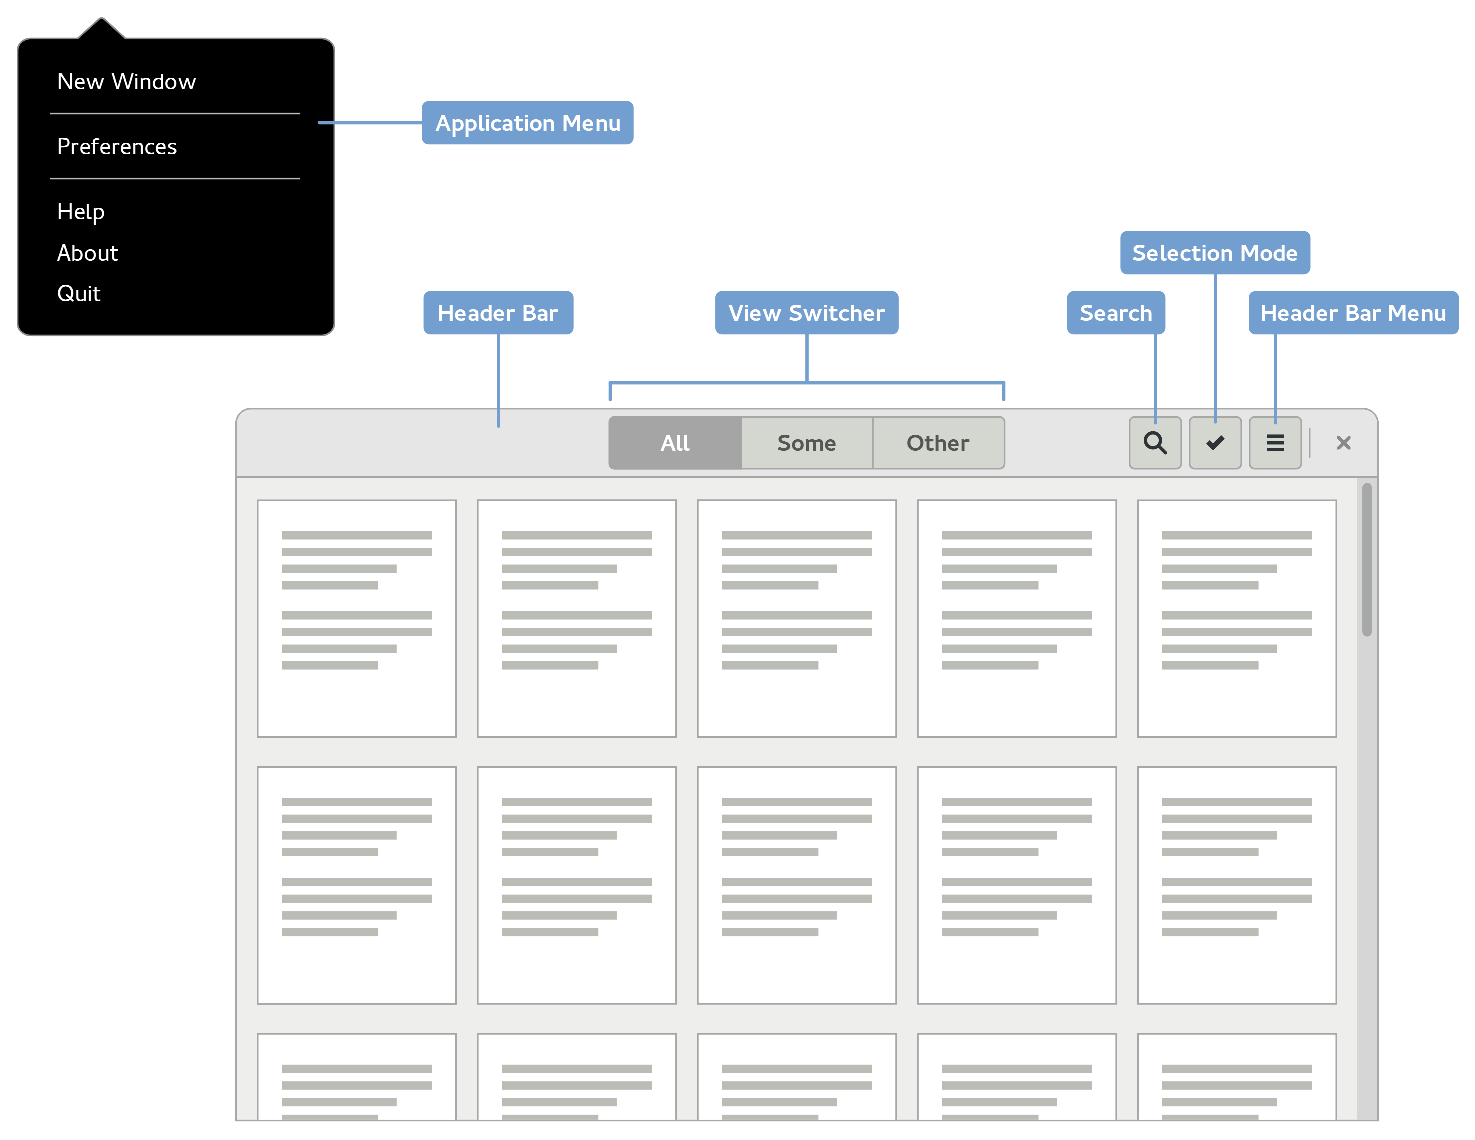
\includegraphics[width=\textwidth]{image/hig/patterns.eps}
    \label{gnome-hig-patterns}
    \fonte{GNOME 3.16 HIG - Patterns}
  \end{center}
\end{figure}


\section{Configuração do Ambiente de Testes}

O projeto GNOME disponibiliza imagens oficiais de um sistema operacional Linux
com todos os pacotes necessários para uma experiência GNOME pré instados e
configurados. Sua utilização trouxe facilidade e consistência nos testes
efetuados.

Dentre as versões disponíveis foram selecionadas :

\begin{center}
    \begin{tabularx}{\textwidth}{ | l | l | l | X | }
    \hline
    Versão do GNOME & Data de Modificação & Nome do arquivo & Soma de Verificação \\
    \hline
    3.6.0 & 08/10/2012 & GNOME-3.6.0.iso       & MD5    753c99ce2342f658 
                                                        65c1f74bc3722e44 \\
    \hline
    3.16  & 25/03/2015 & gnome-3.16.x86-64.iso & SHA256 4a6185a0aca89f15 
                                                        8f769d76d5a0086f 
                                                        0f1e9d709a5d80cd 
                                                        cf2b0d52d67ab2b2 \\
    \hline
    \end{tabularx}
\end{center}

Todas aplicações foram analisadas na versão publicada, sem alterações na
configuração do sistema, troca de temas, fontes, etc. O ambiente virtual foi
provisionado utilizando o software Oracle VM VirtualBox 4.3.26 na seguinte
configuração de máquina:

\begin{center}
    \begin{tabular}{ | l | l | }
    \hline
    \multicolumn{2}{| l |}{Máquina} \\
    \hline
    Memória Base  & 4096MB \\
    Processadores & 2 \\
    Aceleração    & VT-x/AMD-V, Nested Paging, PAE/NX \\
    \hline
    \multicolumn{2}{| l |}{Vídeo} \\
    \hline
    Memória       & 128MB \\
    Aceleração    & 3D \\
    \hline
    \multicolumn{2}{| l |}{Sistema Operacional} \\
    \hline
    Tipo         & Linux \\
    Versão       & Fedora \\
    \hline
    \end{tabular}
\end{center}

